\documentclass[a4paper]{scrartcl}
\usepackage[utf8]{inputenc}
\usepackage[english]{babel}
\usepackage{graphicx}
\usepackage{lastpage}
\usepackage{pgf}
\usepackage{wrapfig}
\usepackage{fancyvrb}
\usepackage{fancyhdr}
\usepackage{float}
\pagestyle{fancy}

% Create header and footer
\headheight 27pt
\pagestyle{fancyplain}
\lhead{\footnotesize{Data Storage Paradigms, IV1351}}
\chead{\footnotesize{Project Report}}
\rhead{}
\lfoot{}
\cfoot{\thepage\ (\pageref{LastPage})}
\rfoot{}

\title{Project Report Task 2}
\subtitle{Data Storage Paradigms, IV1351}
\author{}
\date{2024-11-21}

\begin{document}

\maketitle
\noindent\textbf{Project members:} \\ \hfill
Jonathan Värild, varild@kth.se \\ \hfill
Oscar Caddeo, ocaddeo@kth.se \\ \hfill
Elias Holm, eliholm@kth.se \\ \hfill

\section*{Declaration:}

By submitting this assignment, it is hereby declared that all group members listed above have contributed to the solution. It is also declared that all project members fully understand all parts of the final solution and can explain it upon request.

It is furthermore declared that the solution below is a contribution by the project members only, and specifically that no part of the solution has been copied from any other source (except for lecture slides at the course IV1351), no part of the solution has been provided by someone not listed as a project member above, and no part of the solution has been generated by a system.

\section{Introduction}


\section{Literature Study}


\section{Method}

To create a Logical and Physical Model that accurately represents the requirements of the Soundgood Music School the diagram editor Astah Proffesional was used and the diagram made using IE notation. The Logical and Physical Model was created based on the previous Conceptual model and the approach  of converting it consisted of several steps:

\begin{enumerate}
    \item \textbf{Create tables and columns for entities and attributes}:
  Tables were created for each of the entities and columns within the tables for each attribute. For attributes with cardinality higher than one, separate tables had to be created but this had been considered when creating the Conceptual model so only one change had to be made with an additional table for siblings.

    \item \textbf{Specify types and add constraints}:
  After all tables and columns had been created, types where specified for each column. All primary key id:s where set to 'INT ALWAYS GENERATED AS IDENTITY' for example. Constraints such as NOT NULL and UNIQUE where also added and cardinality specified between tables.

    \item \textbf{Define Keys, relationships, Triggers, Checks and Constraints}:
  For all tables primary keys where defined as well as foreign keys to form relationships between tables. Checks, constraints and triggers where also added to make sure inserted data does not conflict with the requirements. For example a trigger that rejects rental inserts if a student already has 2 active rentals and a trigger that makes sure one instructor can't be booked on different activities during the same timeslot.

    \item \textbf{Normalization}:
  Finally the model was normalized to 3NF since the group decided that was sufficient for the model and any more normalization would only complicate the model. It was firstly normalized to 1NF by making sure the model only contains atomic values, each column only contains one value of a single type and each table has a unique primary key identifier. To normalize it to 2NF it was made sure that the model does not contain any partial dependecies. The final step to normalize it from 2NF to 3NF was to remove any transitive dependencies.

    \item \textbf{Creating the database}:
  When the model was complete, a database was created in accordance with the model. Creating all the tables, columns as well as all checks, constraints and triggers. After that some mock data was created and inserted into the database to test and the scripts for both creating the database and inserting mock data where revised and then uploaded. With the database and mock data now in place, the database was tested to make sure all constraints worked as intended and that the data the requirements lists were able to be retrieved from the database.

\end{enumerate}

\section{Result}

The result of our combined physical and logical diagram of our database can be seen in Figure 1 below. Its structure is very alike to our Conceptual Model Diagram since it already was fairly normalized and compatible with a database structure. The first table that we implemented was the \textbf{person} which uses an automatically incremented integer ID \textbf{school\_id} as primary key. It is automatically incremented using the built-in SQL feature \textbf{GENERATED ALWAYS AS IDENTITY} which ensures that we can't insert values to it. The \textbf{school\_id} is widely used in the database since it is used to identify different persons. Their personal ID number is only used to identify their \textbf{Person} row with their real life identity. This ensures that we in special cases can update the personal ID number of a person if it were to change for some reason. The table have two checks using regex to ensure that the \textbf{personal\_id\_number} and \textbf{zip\_code} are correctly formatted.

The \textbf{student} table has a relationship with \textbf{contact\_details} which store personal or relative contact details for each person. Each contact details have a unique ID that is also \textbf{GENERATED ALWAYS AS IDENTITY}. This is also the primary key of each contact details. Since we don't require both a phone number and an email address we have added a check that ensures they are not null at the same time.

Next, we have the tables \textbf{instructor} and \textbf{student} which uses a foreign key to person which connects them. This allows us to divide each person into roles and also apply additional columns or relations to each role such as \textbf{can\_teach\_ensamble} or the table \textbf{sibling}. The \textbf{instructor} and \textbf{student} row will be automatically deleted if the \textbf{person} reference is deleted since it is defined as \textbf{ON DELETE CASCADE}.

One of our main issues with the Conceptual Diagram Model was that we didn't think about that 3 students with 3 different parents may not be siblings with everyone. For example, student 1 may be sibling with student 2 which share the same mother and the same father. At the same time, student 3 may also be sibling with student 2 by sharing father. Sibling 1 and 2 may however have different fathers and mothers which don't make them siblings. This made it impossible for them all to share a single sibling ID that groups them together. To fix this, we implemented a new table called \textbf{sibling} that takes two foreign keys which both are \textbf{student\_school\_id}s which can link two students together as siblings. To ensure that you cannot insert bidirectional data we created a trigger which automatically ensures the first school ID is the smallest one and the second school ID is the largest one. These two IDs build the primary key which ensures only one sibling relation can be saved for two students. We also added a check to ensure that a student cannot be a sibling with themselves. If any of the students are removed from the database, the sibling relationship is automatically removed since both foreign keys are defined as \textbf{ON DELETE CASCADE}.

The \textbf{instructor} table has a relationship with \textbf{instrument\_skill} which defines what instrument skills each instructor has. The \textbf{instrument\_skill} table in turn has a foreign key to \textbf{instructor} which links them together. If the \textbf{instructor} row is deleted, so is the \textbf{instrument\_skill} row since the foreign key is defined as \textbf{ON DELETE CASCADE}. The \textbf{skill\_level} column also has a check which enforces that the value is between 1 and 3 indicating the different skill levels beginner, intermediate, and advanced.

Next, we have the \textbf{activity} table which store general information about all types of activities like individual lessons, group lessons and ensembles. This table also has a generated integer ID. It has a check to ensure that the start and end time of each activity is in the correct order. The \textbf{activity} table also has relationships with the \textbf{lesson\_individual}, \textbf{lesson\_group}, and \textbf{ensamble} tables. These tables help to group each activity into the different types. This is also a small change from our conceptual model diagram which used Lesson to define both an individual and group lesson but with different values to their min and max student attributes. To ensure that we don't have a table with a lot of NULL values for min and max students, we decided to split the tables up instead which removes this need. Both \textbf{lesson\_group} and \textbf{ensamble} share checks to ensure the min students are above 1 and that max students is larger that the min students. All 3 tables share \textbf{ON DELETE CASCADE} on \textbf{activity\_id} which ensures that their row is deleted if the activity row is deleted. The tables \textbf{lesson\_individual} and \textbf{lesson\_group} share the check to ensure that the skill level is between 1 and 3 in the same way as it's defined for the \textbf{instrument\_skill} table. The \textbf{activity} table has \textbf{ON DELETE RESTRICT} on all foreign keys to ensure that these are not removed before all their references are replaced or removed. The \textbf{activity} table also have a trigger that ensures a instructor isn't booked on overlapping times since the instructor can't be at two places at the same time.

The \textbf{activity} table also has a relationship to the \textbf{location} table which is a table of all possible locations where you may host an activity. The \textbf{location} table has a check to ensure that not both \textbf{room\_name} or \textbf{video\_link} are NULL since a location may be either physical, online, or both.

Next we have the \textbf{pricing} table which hold pricing information for each activity type based on its type and skill level. It also holds extra information such as sibling discount percentage, if its active and a unique ID. This fulfills the requirement to be able and update the price of a certain activity but still be able to see the old price after its updated. Each activity store the id to the pricing row that was active at that time. If you wish to update the pricing you simply set the current row's to active column to false and insert a new row matching the same activity and skill level. The \textbf{pricing} table also has a number of checks such as that \textbf{activity\_type} is between 1 and 3 which indicates individual lesson, group lesson, and ensemble. It has a check to ensure skill level is between 1 and 3, that the price isn't negative, and that the sibling discount is a number between 1-100 indicated by a discount percentage.

The \textbf{booking} table has a relationship with both the \textbf{activity} and the \textbf{student} table and is used to store what activities each student is booked for. Both foreign keys are set to \textbf{ON DELETE CASCADE} which ensures that a booking is removed if its student or activity is removed.

Looking in the other direction of \textbf{person} we have the \textbf{rental} table which keeps track of all rentals made by each student. It has foreign keys to the student \textbf{school\_id} and instrument \textbf{inventory\_id} which are defined as \textbf{ON DELETE CASCADE} since there is no meaning to keep track of a rental that cannot be linked to a person or instrument. The table is linked to person to ensure that both students and instructors should be able to make rentals. To fulfill the requirement on that each student only should be able to have two active rentals we have added a trigger that checks this before a row is inserted or updated. Another check ensures that the rental time does not exceed 12 months.

Finally, we have the \textbf{instrument} table which store information about all instruments that the school has in inventory available for rental. All instruments of the same brand and model are stored in the same row and are instead kept track of using a \textbf{quantity} column that defines how many instruments there are. The table has two checks to ensure that the quantity and price is over 0.

\begin{figure}[H]
  \begin{center}
    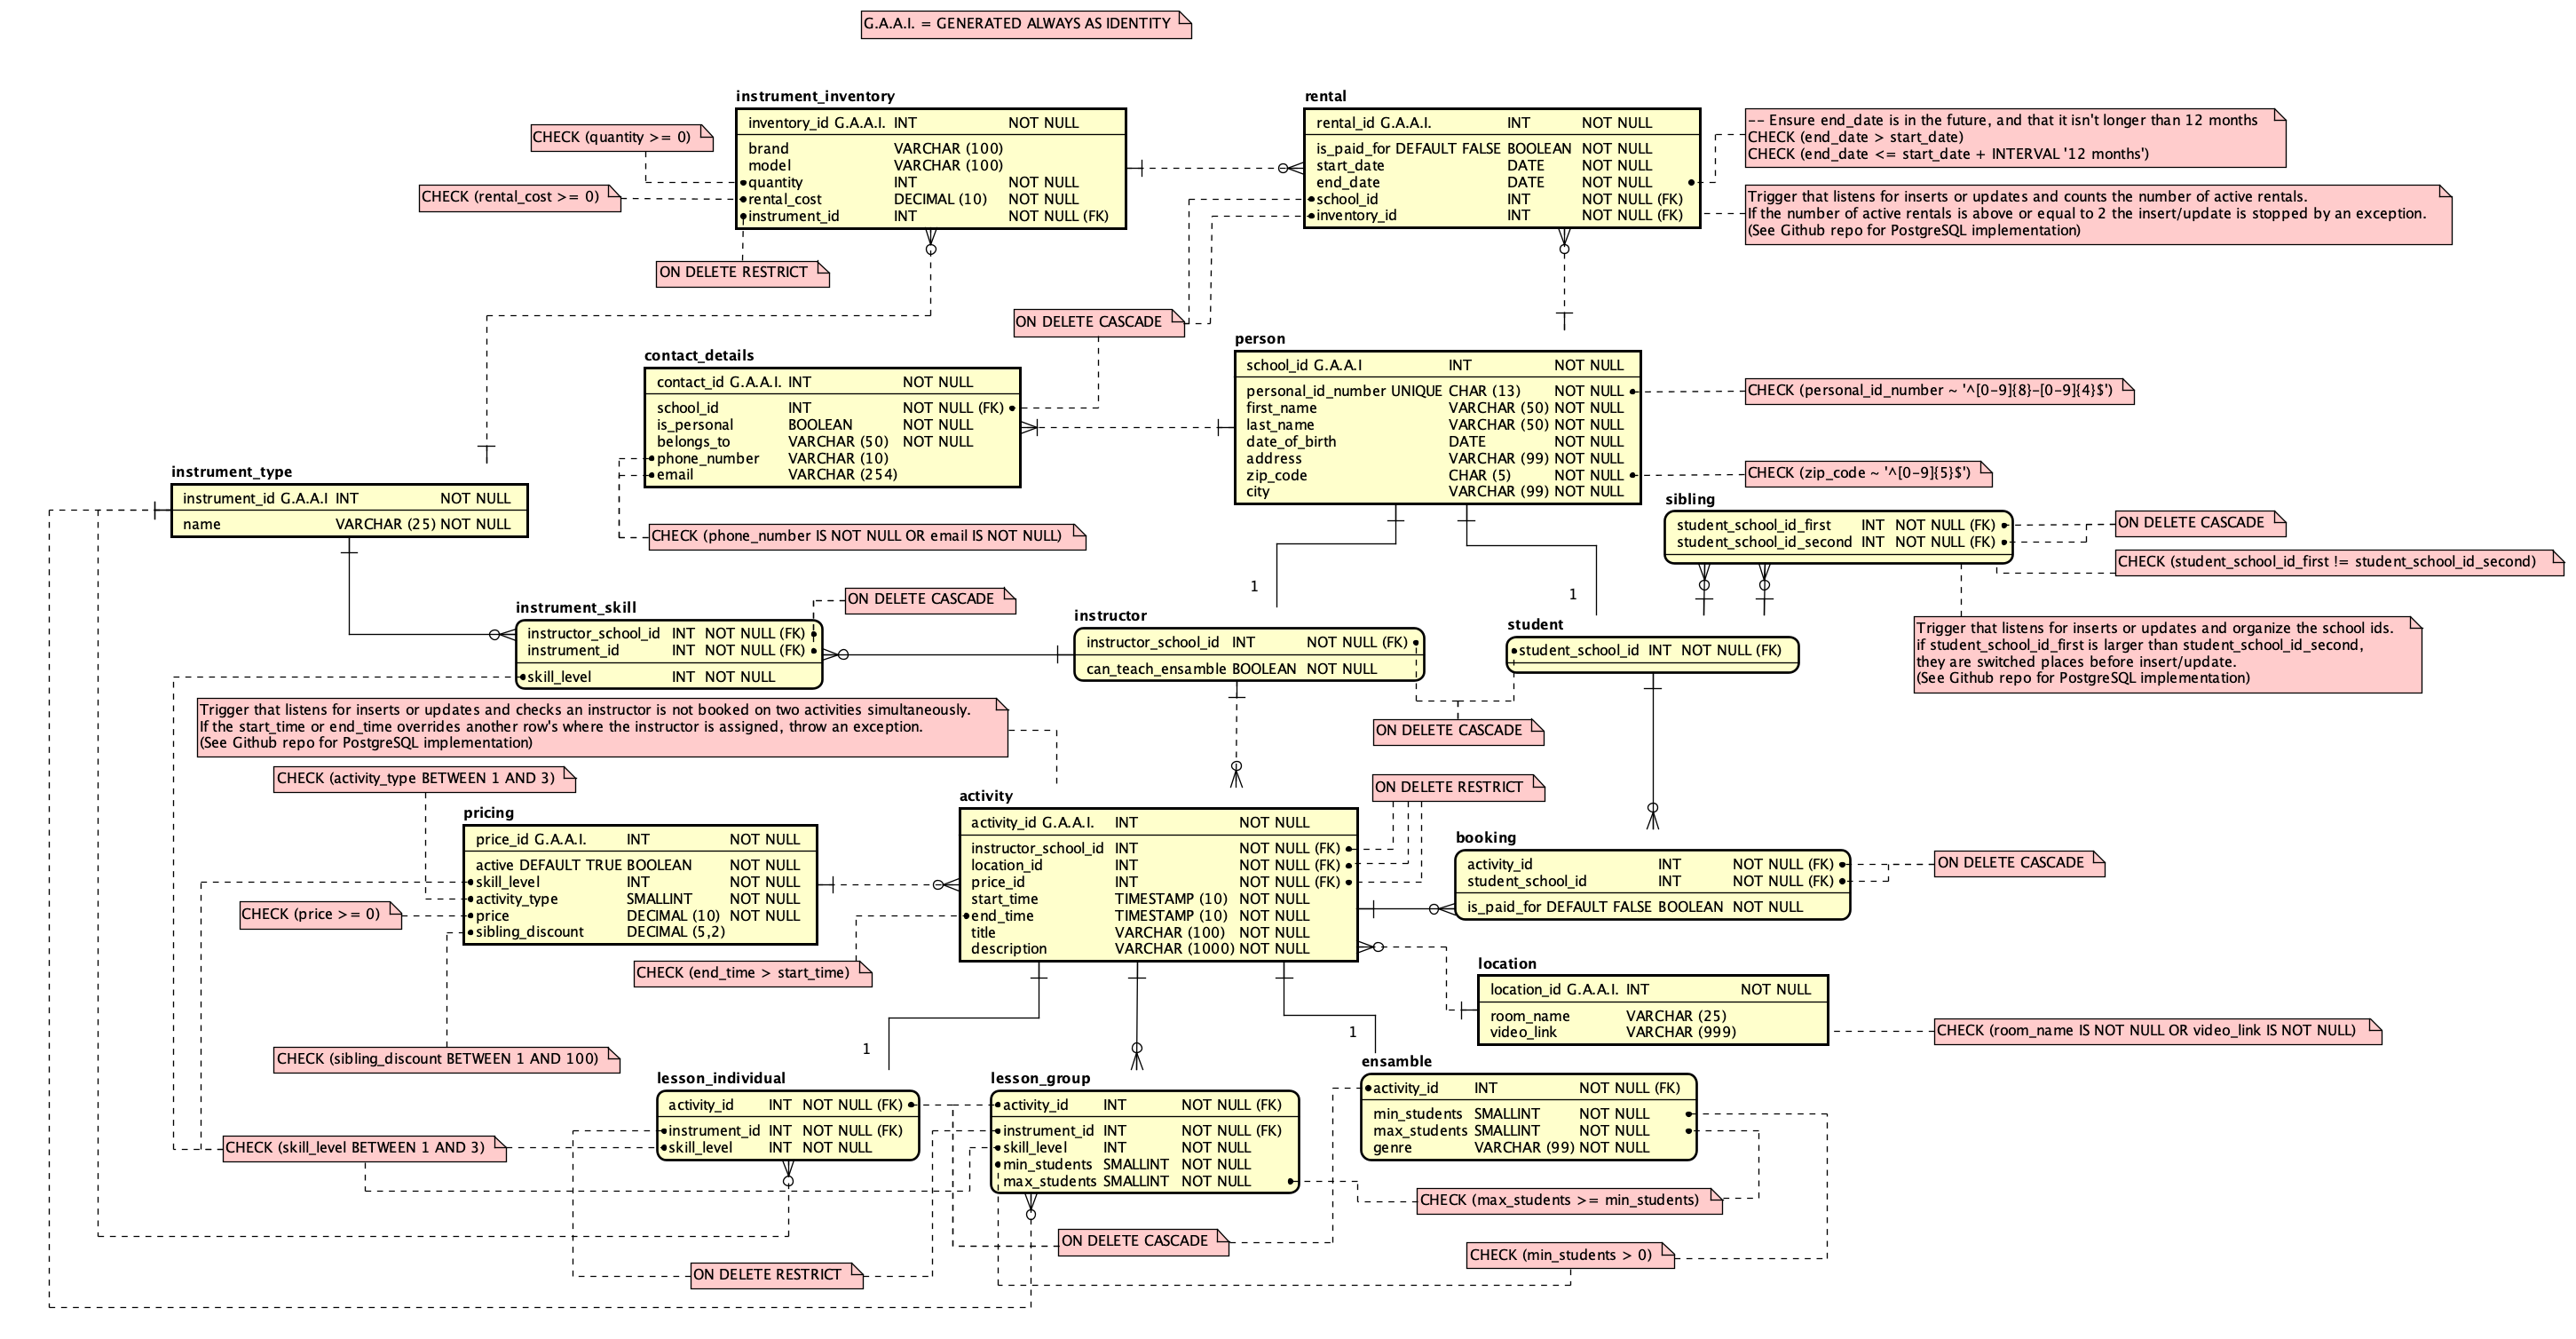
\includegraphics[scale=0.18]{Diagram Picture.png}
    \caption{The physical/logical diagram that we came up with.}
    \label{fig:diag}
  \end{center}
\end{figure}

\section{Discussion}

\subsection{Question 1}

\subsection{Question 2}

\subsection{Question 3 ...}

\section{Comments About the Course}


\end{document}
